\documentclass{beamer}

\renewcommand{\arraystretch}{1.5}
\usepackage{graphicx}
\usepackage{booktabs}\title[EE241 Midterm Report]{EE241 Midterm Report}
\newcommand{\gwidth}[0]{0.7\textwidth}
\author{Albert Magyar, David Biancolin, Jack Koenig}
\date{\today}

\begin{document}
\begin{frame}
  \titlepage
\end{frame}

\begin{frame}{Status}
\end{frame}

\begin{frame}{Creating a baseline design point}
  \begin{itemize}
  \item Store extra bit (ZIB) indicating if byte is zero
  \item Locally gate wordline if ZIB set
  \item Adds area, leakage, and delay overhead
  \end{itemize}
    \begin{figure}
    \centering
    \includegraphics[width=\gwidth]{figs/dzc_impl.pdf}
  \end{figure}
\end{frame}

\begin{frame}{Creating a baseline design point}
  \begin{itemize}
  \item Implement DZC SRAM layout in Virtuoso
  \item Work can be reused for more complex compression
  \item Currently tiling pre-supplied 6T bitcell
  \end{itemize}
    \begin{figure}
    \centering
    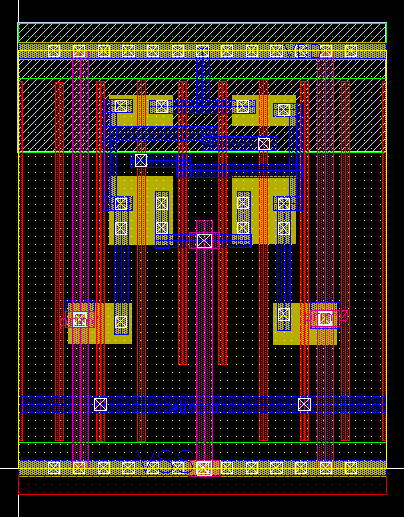
\includegraphics[width=0.4\textwidth]{figs/bitcell.pdf}
  \end{figure}
\end{frame}

\end{document}
